\documentclass[
  12pt,
  a4paper,
  parskip,
  openany
]{scrbook}

\usepackage[utf8]{inputenc}
\usepackage[english]{babel}

\usepackage[hidelinks]{hyperref}
\usepackage{enumitem}
\usepackage{suffix}
\usepackage{lipsum}
\usepackage{tabularx}
\usepackage{graphicx}

% Citation packages and options
\usepackage{csquotes}
\usepackage[
  backend=biber,
  style=apa,
  sorting=none
]{biblatex}
\addbibresource{bibliography.bib}

% ===== INDIVIDUAL AUTHORS PER CHAPTER =====
% Source: https://tex.stackexchange.com/a/156865
\newcommand\chapterauthor[1]{\authortoc{#1}\printchapterauthor{#1}}
\WithSuffix\newcommand\chapterauthor*[1]{\printchapterauthor{#1}}

\makeatletter
\newcommand{\printchapterauthor}[1]{%
  {\parindent0pt\vspace*{-25pt}%
  \linespread{1.1}\large#1%
  \par\nobreak\vspace*{35pt}}
  \@afterheading%
}
\newcommand{\authortoc}[1]{%
  \addtocontents{toc}{\vskip-10pt}%
  \addtocontents{toc}{%
    \protect\contentsline{chapter}%
    {\hskip1.3em\mdseries\protect\scriptsize#1}{}{}}
  \addtocontents{toc}{\vskip5pt}%
}
\makeatother
% ==========================================


\title{NoSQL Databases}
\author{Daniel Rutz and Leon Schürmann (Eds.)}
\date{\today}

\begin{document}

\maketitle
\tableofcontents

\chapter{Key Value Introduction}
\chapterauthor{Vanessa Jörns, Tobias Schiffmann and Victor Veal}
Key-value databases or key-value stores are a classification of NoSQL databases. 
The idea of key-value stores is to collect a key  for every data set. Each set that is stored in the database can be accessed by the key. Therefore the key needs to be distinct, whether in a namespace or in the whole system. The database system has no pattern for the values which is why it is not  necessary to know about the type of the values that are stored. This feature enables easy storage of any kind of data like serialized structures, XML, text data, files...  (\cite{keyValueIntro}).

However, there are also disadvantages of this database management type. In terms of operational actions like querying through the data, as one would do in relational database management systems, key-value databases only provide simple operations like get, put and delete. As a result of this constraint, data querying must be handled at the application level. 

Another difference to relational databases are the use cases. 
 For simple applications, which only require a system that is able to store and manage data (e.g. update entries, join tables), is capable of representing real-world entities and describes relationships, relational databases should be used. Key-value databases should rather be chosen if the application or the system requires a good performance since key-value solutions are faster than relational database systems (\cite{keyValueUsecase}).
 
For instance, an online application that is only responsible to enable quick access to a profile, does not need to interact with entries of the profile itself. It should rather guarantee that the user of the application can easily find the profile by providing the corresponding key. To enable a quick access of the profile, it would be enough to only search for the unique ID of the profile instead of querying across several attributes of the data set.

Nevertheless, not all key-value solutions are similar designed. There are a lot of different systems today. In the following chapters some database management systems will be introduced. The focus will be on providing the reader a quick overview about the different systems, how they distinguish from each other and how to use them.

The first system that will be explained is Hazelcast which gives an overview of the the basic characteristics including a cheat sheet with needed commands. The next section talks about Redis and the basic features as well as in-memory computing. Last but not least the Key Value chapter is finished with a section about Riak. 


% eventuell Bild
% [1] https://en.wikipedia.org/wiki/Key-value_database#/media/File:KeyValue.PNG

\chapter{Hazelcast}
\chapterauthor{Vanessa Jörns, Tobias Schiffmann and Victor Veal}

\section{Hazelcast Introduction}

Hazelcast is a company that is developing an in-memory computing platform consisting of Hazelcast IMDG, Hazelcast Jet and Hazelcast Cloud. “Hazelcast Jet is an embeddable, distributed computing platform for fast processing of big data sets”. It is built on the foundation of Hazelcast IMDG on which this chapter focuses (\cite{hazelcast}).

An in-memory data grid (IMDG) is a rather new concept where data is stored in the main memories of a computing cluster. One of the main aspects is the ability to automatically scale and rebalance the cluster when decreasing or increasing in size. Here the data is partitioned equally across the cluster nodes. IMDGs are usually used for implementing distributed and scalable applications since they provide distributed versions of the basic data structures (\cite{tasci2015}). Hazelcast IMDG is open source and implemented in Java. However, there are also existing API’s for C/C++, .NET, REST, Python, Go and Node.js.

As Hazelcast is designed to be lightweight and easy to use, it can be downloaded as a compact library (JAR) and can be used by simply adding this JAR file to the classpath. With Java as the only dependency there is no need to install any software (\cite{hazelcastmanual}).

Firstly, the features of Hazelcast are specified and distinguished from other key-value solutions. The next section talks about the CAP theorem and how it applies to Hazelcast. After that a short manual for implementing Hazelcast for own applications is provided. This inlcudes a basic set up as well as a configuration. For reference a cheat sheet with the most important commands is included. In the end, the whole chapter about Hazelcast is concluded and the advantages and disadvantages are analyzed. 
\section{Specification}
Hazelcast consists of many same or similar features like other key value databases and IMDGs. However, there are some major features which describe Hazelcast’s distinctive strengths.
The first and one of the main characteristics is that Hazelcast completely computes in-memory rather than storage based.  This makes Hazelcast extremely fast but also volatile.

Another major feature is that Hazelcast relies on clustering with the approach of a “masterless nature” of the nodes. This means that each node in the cluster has the exact same functionality and operates in a peer-to-peer manner (\cite{johns2015}). So unlikely other NoSQL databases, there is no master and slave hence there is no single point of failure. All nodes are responsible for the same proportion of processing and storing (\cite{hazelcastmanual}). The oldest node of the cluster automatically becomes the “de facto leader” and manages the distribution of the data for joining nodes. Since the data is redistributed for every joining or exiting node, the cluster rebalances automatically and thus makes Hazelcast simple to set up and configure.

As Hazelcast consists of the basic features of an in-memory data grid, the data and therefore the load is equally spread across the cluster. Here each node is the owner and holds a number of partitions of the overall data.
Therefore, saturation of a cluster can simply be overcome by adding more nodes to the cluster. The cluster is then rebalanced and the load for each node decreases. This means scaling is easy and fast which makes Hazelcast suitable for handling big amounts of data.
Nevertheless, since Hazelcast persists data entirely in-memory, it has the main drawback that data will be lost with a node shutting down. To prevent the overall cluster of losing the data a failing node has held, Hazelcast distributes backups of each data partition among multiple other members. This means in case of a node shut down, another node will have a backup of the data and the cluster can be rebalanced without suffering any data loss and downtime (\cite{johns2015}).
\begin{figure}[H]
    \centering
    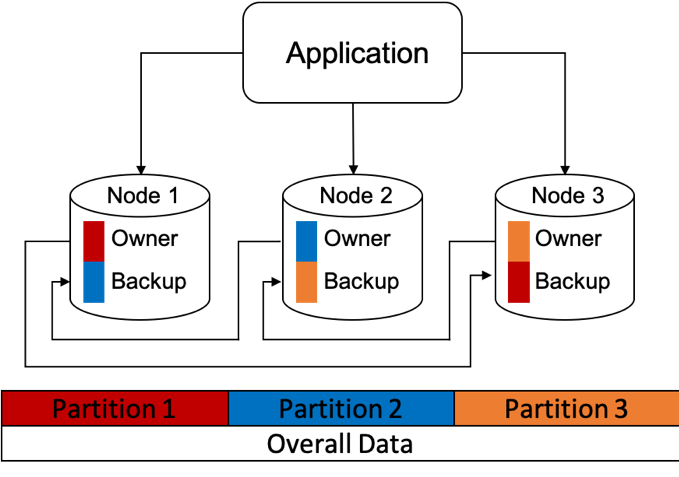
\includegraphics[scale=0.6]{content/images/hazelcast-nodes.png}
    \caption{Hazelcast Nodes (\cite{johns2015})}
\end{figure}
This illustration shows the cluster structure as described above. It explains how the data is partitioned in equal parts and spread across the cluster as well as the replication of the data for backup. This is just a simplified version of the structure with only three nodes. In practice each node would be responsible for multiple subsets of the data and not just one data partition. So, for instance in order to get the data of Partition 1, the application has to communicate with Node 1. The distribution of the data is dynamic and which node is responsible for which subset of data usually changes over time. Hence, the allocation is an internal operational detail and the application as well as the user usually does not need to know it.
Moreover, Hazelcast supports various distributed collectors, features and processors. Besides storing the data in-memory distributed on many nodes, it is possible to load data from diverse sources into varying structures, communicate across the cluster by sending messages and to use the stored data for analytical processing (\cite{johns2015}).


\section{Hazelcast and the CAP theorem}
As Hazelcast enables data storage for distributed systems, it may be interesting how the CAP theorem applies to it. According to the chapters before, Hazelcast offers a storage mechanism that distributes data across several nodes. Therefore the first aspect out of the CAP theorem is network partitioning. According to the article \textit{Jepsen Analysis on Hazelcast 3.8.3} (\cite{hazelcastCP}), Hazelcast is a PA system which means that it favours availability over consistency. Due to the fact that data is partitioned, the problem of keeping the data consistent over the whole system occurs. For example, if the user inserts a new entry to a cluster, the whole systems needs to update this info so that the same information can be provided from all nodes. This problem of having several nodes storing inconsistent data is called split brain in an In-Memory Data Grid system.

Hazelcast offers a method that should avoid split brain. In the so called "Split Brain Protection" a minimum number of nodes is set on which write or read operations are prevented. If a split brain happens, any sub-clusters that have a lower number of nodes than the minimum number are prevented from accepting write operations. Nevertheless, this method only reduces the time of inconsistency. Therefore it does not completely avoid the inconsistent state of the system (\cite{hazelcastCP}).

Recently, the Hazelcast company has announced the ability to provide a solution that supports both PA (availability over consistency) and PC (constistency over availability). This feature should allow the user to adapt more flexibly to the requirements of the application. So far, there are too less resources that can describe this new feature of Hazelcast which is why this paper is currently not able to report about it (\cite{hazelcastCAP}).

\section{Implementation}
\subsection*{Getting Started}
As already mentioned Hazelcast is designed to be easy to use and therefore only require a few steps to set it up running.
First of all, the Hazelcast package has to be downloaded, for example from the official website (\cite{hazelcast:hazelcastDownload}). The package is offered in a compressed data format and has to be extracted afterwards.

Hazelcast does not need any software installations. It is written in Java and therefore the platform to run Hazelcast on needs to be able to execute Java code. To do so a Java Development Kit has to be ready to use which can be gathered from the Oracle website. After ensuring Java code to run, Hazelcast is ready to be used.

The console application is an easy way to get in touch with Hazelcast and experience the software. It can be started by executing the \texttt{console} scripts in the \texttt{demo/} directory from a terminal. Hazelcast creates a new member which will either create a new cluster or will join a cluster if there already exists one. The cluster can than be filled by typing the commands as the following example shows.
\begin{flushleft}
\begin{figure}[h]
    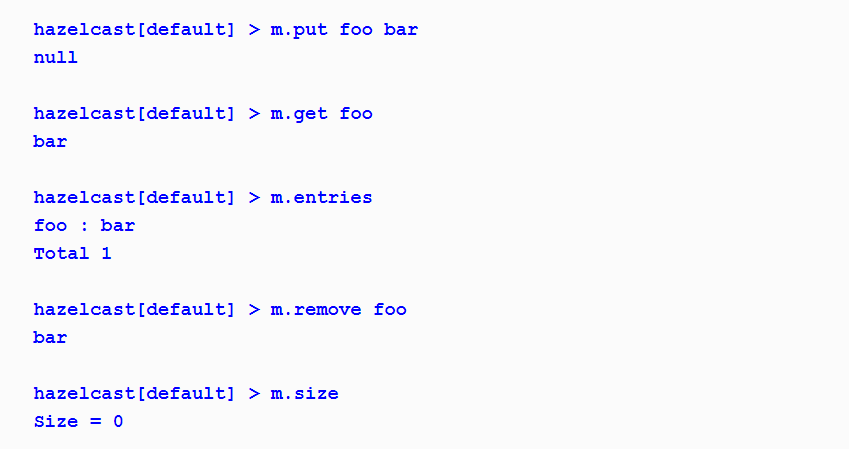
\includegraphics{content/images/hazelcastPut.PNG} 
    \caption{Hazelcast Basic Commands (\cite{johns2015})}
\end{figure}
\end{flushleft}
When executing the scripts in another window, Hazelcast shows how the new member joins the cluster and displays the two members and there addresses after a short period of time.

\begin{flushleft}
\begin{figure}[h]
    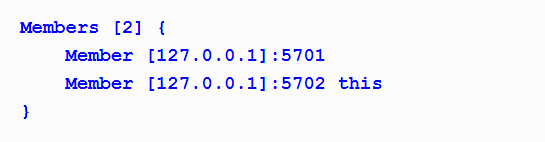
\includegraphics{content/images/hazelcastMembers.PNG}
    \caption{Example Member List (\cite{johns2015})}
\end{figure}
\end{flushleft}
Now the data is spread across the members. They both own a particular partition of the data and store the other part as backup.

When closing one terminal to test Hazelcast's reaction to a cluster node failure, the remaining member tries to reestablish the connection to the closed one, but without success. The terminal will than display the process of repartitioning the cluster and prints a statement when it finishes.
\subsection*{Members and Clients}
Besides the console application Hazelcast also provides the opportunity to include the Hazelcast package in your code. For Java there is a package for members and one for clients provided. Other programming languages only have clients to work with. The difference between clients and members is that clients do not hold data. They connect to Hazelcast cluster members and access the data on that way for read and write operations (\cite{hazelcastmanual}). If Hazelcast has to be set up for an application in C++ for example, the scripts in the \texttt{demo/} directory can be used to start a cluster member without needing to create a java application. The C++ application than has to include the Hazelcast package and can access or create the data via the member.
\subsection*{Configuration}
Hazelcast offers an XML file to adjust certain configurations in the \texttt{bin/} directory.
It is possible to change the amount of backups and also the types of backups. There are normal backups which are synchronized and therefore lock the data in case it is manipulated. All other nodes have to wait until the data is changed in all backups and the changes are confirmed by the nodes which hold the backups. Additionally, there are asynchronous backups. They do not lock any data and therefore bring a performance increase because the nodes do not have to wait for them to confirm the changes. On the other hand, it brings the risk of inconsistent data. Nodes could access data which are no longer valid because the changes were not made on all backups after a manipulation took place.

In general, increasing the number of backups will increase the read performance because the data can be read on different nodes in parallel. The costs for this advantage are either bad write performance in case of normal backups or inconsistency in case of asynchronous backups.

Furthermore Hazelcast provides configurations about how big a particular data structure can grow and how to act when there is no more space left. 
\begin{flushleft}
\begin{figure}[h]
    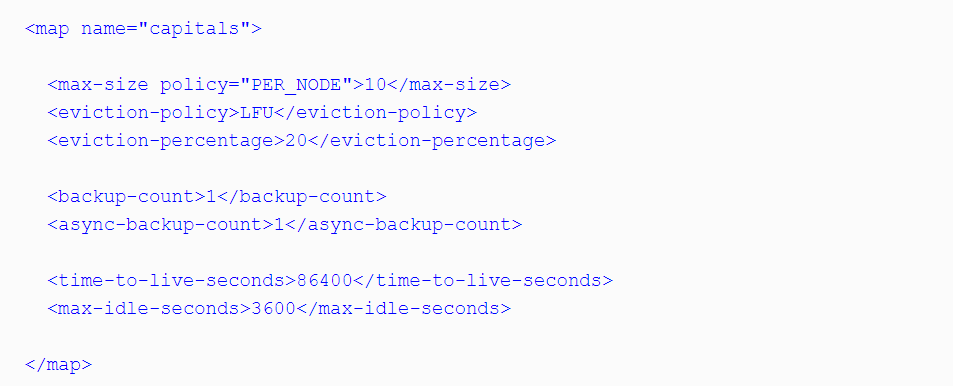
\includegraphics{content/images/hazelcastXML.PNG}
    \caption{Hazelcast Configuration (\cite{johns2015})}
\end{figure}
\end{flushleft}
In this example the map called \textit{"capitals"} has a maximum size of 10 items per node. When reaching this maximum, 20 percent of the data will be freed according to the principle of Least Frequently Used (LFU). One synchronous and one asynchronous backup will be created and the time to live for data sets is set. This means that data will be deleted after this amount of seconds goes by. In contrast to this, setting the maximum idle time will only delete a data set when it is not accessed after a certain amount of seconds.
\citeauthor{johns2015} and the Hazelcast websites provide more information about configuration and go more in detail.

\section{Cheat Sheet}
\subsection*{General commands}
\begin{tabular}{|p{0.3\textwidth}|p{0.7\textwidth}|}
    \hline
    \texttt{echo true|false} & turns on/off echo of commands (default false)\\\hline
    \texttt{silent true|false} & turns on/off silent of command output (default false)\\\hline
    \texttt{\# <number> <command>}& repeats \texttt{<number>} time \texttt{<command>}, replace \$i in \texttt{<command>} with current iteration (0...\texttt{<number-1>)}\\\hline
    \texttt{\& <number> <command>}& forks \texttt{<number>} threads to execute \texttt{<command>}, replace \$t in \texttt{<command>} with current thread number ((0...\texttt{<number-1>)})\\\hline
    \texttt{jvm} & displays info about the runtime\\\hline
    \texttt{who} & displays info about the cluster\\\hline
    \texttt{whoami} & displays info about this cluster member\\\hline
    \texttt{ns} \texttt{<string>} & switch the namespace for using the distributed queue/map/set/list \texttt{<string>} \newline (default value = "\texttt{default}")\\\hline
    \texttt{@ <file>} & executes the given \texttt{file} script. Use '//' for comments in the script\\\hline
\end{tabular}
\subsection*{Queue commands}
\begin{tabular}{|p{0.3\textwidth}|p{0.7\textwidth}|}
    \hline
    \texttt{q.offer <string>} & adds a string object to the queue\\\hline
    \texttt{q.poll} & takes an object from the queue\\\hline
    \texttt{q.offermany <number> [<size>]} & adds indicated number of string objects to the queue ('\texttt{obj<i>}' or \texttt{byte[<size>]})\\\hline
    \texttt{q.pollmany <number>} & takes indicated number of objects from the queue\\\hline
    \texttt{q.iterator [remove]} & iterates/displays the queue, remove if specified\\\hline
    \texttt{q.size} & adds a string object to the queue\\\hline
    \texttt{q.clear} & clears the queue\\\hline
\end{tabular}
\subsection*{Set commands}
\begin{tabular}{|p{0.3\textwidth}|p{0.7\textwidth}|}
    \hline
    \texttt{s.add <string>} & adds a string object to the set\\\hline
    \texttt{s.remove <string>} & removes the string object from the set\\\hline
    \texttt{s.addmany <number>} & adds indicated number of string objects to the set ('\texttt{obj<i>}')\\\hline
    \texttt{s.removemany <number>} & takes indicated number of objects from the set\\\hline
    \texttt{s.iterator [remove] } & iterates/displays the set, removes if specified\\\hline
    \texttt{s.size} & size of the set\\\hline
    \texttt{s.clear} & clears the set\\\hline
\end{tabular}
\subsection*{List commands}
\begin{tabular}{|p{0.3\textwidth}|p{0.7\textwidth}|}
    \hline
    \texttt{l.add <string>} & adds string to the list\\\hline
    \texttt{l.add <index> <string>} & adds string at a certain index\\\hline
    \texttt{l.contains <string>} & checks if list contains \texttt{<string>}\\\hline
    \texttt{l.remove <string>} & removes \texttt{<string>} from list\\\hline
    \texttt{l.remove <index>} & removes element at \texttt{<index>} from list\\\hline
    \texttt{l.set <index> <string>} & replaces value at \texttt{<index>} with \texttt{<string>}\\\hline
    \texttt{l.iterator [remove]} & iterates/displays the list\\\hline
    \texttt{l.size} & size of list\\\hline
    \texttt{l.clear} & clears list\\\hline
\end{tabular}
\subsection*{Map commands}
\begin{tabular}{|p{0.3\textwidth}|p{0.7\textwidth}|}
    \hline
    \texttt{m.put <key> <value>} & puts an entry to the map\\\hline
    \texttt{m.remove <key>} & removes the entry of given key from the map\\\hline
    \texttt{m.get <key>} & returns the value of given key from the map\\\hline
    \texttt{m.putmany <number> [<size>] [<index>]} & puts indicated number of entries to the map ('\texttt{key<i>}':\texttt{byte[<size>]}, \texttt{<index>+(0..<number>})\\\hline
    \texttt{m.removemany <number> [<index>]} & removes indicated number of entries from the map ('\texttt{key<i>}', \texttt{<index>+(0..<number>})\\\hline
    \texttt{m.keys} & iterates/displays the keys of the map\\\hline
    \texttt{m.values} & iterates/displays the values of the map\\\hline
    \texttt{m.entries} & iterates/displays the entries of the map\\\hline
    \texttt{m.iterator [remove]} & iterates/displays the keys of the map, remove if specified\\\hline
    \texttt{m.size} & size of the map\\\hline
    \texttt{m.localSize} & local size of the map\\\hline
    \texttt{m.clear} & clears the map\\\hline
    \texttt{m.destroy} & destroys the map\\\hline
    \texttt{m.lock <key>} & locks the key\\\hline
    \texttt{m.trylock <key>} & tries to lock the key and returns immediately\\\hline
    \texttt{m.trylock <key> <time>} & tries to lock the key within given seconds\\\hline
    \texttt{m.unlock <key>} & unlocks the key\\\hline
    \texttt{m.stats} & shows the local stats of the map\\\hline
\end{tabular}
\subsection*{MultiMap commands}
\begin{tabular}{|p{0.3\textwidth}|p{0.7\textwidth}|}
    \hline
    \texttt{mm.put <key> <value>} & puts an entry to the multimap\\\hline
    \texttt{mm.get <key>} & returns the value of given key from the multimap\\\hline
    \texttt{mm.size} & size of the multimap\\\hline
    \texttt{mm.clear} & clears the multimap\\\hline
    \texttt{mm.destroy} & destroys the multimap\\\hline
    \texttt{mm.iterator [remove]} & iterates the keys of the multimap, remove if specified\\\hline
    \texttt{mm.keys} & iterates/displays the keys of the multimap\\\hline
    \texttt{mm.values} & iterates/displays the values of the multimap\\\hline
    \texttt{mm.entries} & iterates/displays the entries of the multimap\\\hline
    \texttt{mm.lock <key>} & locks the key\\\hline
    \texttt{mm.trylock <key>} & tries to lock the key and returns immediately\\\hline
    \texttt{mm.trylock <key> <time>} & tries to lock the key within given seconds\\\hline
    \texttt{mm.unlock <key>} & unlocks the key\\\hline
    \texttt{mm.stats} & shows the local stats of the map\\\hline    
\end{tabular}

\section{Conclusion}

Hazelcast is categorized as a key-value NoSQL solution, but since it is an in-memory data grid there are some main features that should be emphasized which set Hazelcast apart from the ordinary key-value databases.
First of all, one of the key characteristics is its simplicity. As mentioned above, Hazelcast’s only dependency is Java and therefore it can be used by simply downloading the JAR file and including it in the classpath.
Furthermore, the cluster is structured as a peer-to-peer network, meaning there is no master-slave relation which is usually common for NoSQL databases. Each node is responsible for the same amount of data.

Another characteristic is the speed of Hazelcast since it relies on in-memory computing (\cite{hazelcastmanual}). Knowingly in-memory computing also comes with two main downsides: volatility and scalability. Hazelcast, however addresses these issues.
Volatility is solved by keeping the data of the nodes redundant. This means that Hazelcast stores the data of each node on multiple members. So, if one member fails, there is a backup and the whole cluster can be rebalanced and there is no overall loss of the data.
Scalability is achieved by just adding more nodes to the cluster, the data is then automatically rebalanced and the work load for each member decreases.

These main features of Hazelcast also directly conclude some major advantages. To summarize the already mentioned ones, Hazelcast is very easy and fast to install and it is designed to provide fast computing. Additionally, since there is no master-slave concept, there is also no single point of failure. It is easy to scale either up or down and redundant data storage protects from unexpected data loss (\cite{hazelcastnosql}).
Furthermore, in contrast to ordinary key-value databases, Hazelcast is designed for a distributed environment and therefore it is possible to provide an unlimited number of maps and caches per cluster. Another advantage is that Hazelcast can be implemented using multiple threads and thus benefits from all available CPU cores (\cite{hazelcastredis}).

Nevertheless, Hazelcast relying entirely on in-memory processing still comes with the drawback that this kind of storage is temporary. So, in case there is an overall system shut down the data is lost since the backups are stored in the same cluster. In addition, RAM is usually expensive which should be kept in mind when considering scalability.

Regarding the CAP theorem, as discussed above, Hazelcast can be either implemented as an PA or PC system. When using Hazelcast as a PA system, it is neglecting consistency. Meaning the system is not fully consistent all the time. On the other hand, in case of a PC system, it fails to provide continuous availability.
Furthermore, as a PC system the speed of the data grid system relies on the slowest node. If backups are kept synchronously, data is locked until the consistent state is achieved again (\cite{johns2015}). The other nodes will have to wait until this particular block of data is unlocked again.


Hazelcast provides several and detailed manuals online as well as understandable tutorials which makes it easy to adapt Hazelcast for own applications. However, scientific research and benchmarking is very limited.

\printbibliography

\end{document}
